\hypertarget{case-study---replication-of-a-seurat-workflow}{%
\section{Case Study - Replication of a Seurat
workflow}\label{case-study---replication-of-a-seurat-workflow}}

Autoren: Guido Schlögel 00727019 Sonja Tockner 00708717

\hypertarget{introduction}{%
\subsection{Introduction}\label{introduction}}

Replication of results is an important part of science. As it is
important to avoid the replication crisis in data science, we want to
show in this exercise how the Seurat tutorial for single cell RNA
sequencing (scRNA-Seq) can be replicated and adapted to a different
dataset.

scRNA-Seq is chosen as it became an important tool to understand
biological systems, but still lacks standardization (Luecken and Theis
2019).

So what is it and why do we use it.

\hypertarget{advantages-over-bulk-methods}{%
\subsubsection{Advantages over bulk
methods}\label{advantages-over-bulk-methods}}

In Single cell RNA-seq each sequencing library represents a single cell
while Bulk RNA-Seq represents a whole cell population. Within a single
tissue, there are many similar cells that may have specific functions,
which can be addressed with scRNA Seq. Bulk sequencing studies the
genome/transcriptome. The differential gene expression of healthy and
diseased individuals is compared as an average representation, bulk
RNA-seq is used for studying biomarkers and understanding the biology of
diseases. scRNA Seq has several advantages over bulk RNA-seq, including
more accurate prediction of disease, discovery of new cell types, and
the ability to study gene expression in individual cells (e.g., finding
differences in specific cell types).

scRNA Seq enables detailed analysis of individual cells and reveals
cellular heterogeneity. In comparison, the bulk method measures the
average expression across a population of cells and the cellular
heterogeneity is masked. ScRNA Seq provides high resolution and
transcriptional profiling of thousands of individual cells, allows to
understand gene expression at a single cell level and finds differences
within a heterogenous sample. It measures the distribution of the
expression level for each gene across a population of cells. In
comparison, a bulk sample represents many cells where all kinds of RNA
sequences from the sample are extracted without filtering and
enrichment, measuring the average expression level for each gene across
a large population of input cells (e.g., a sample from the same tissue
from different species).

\hypertarget{basic-steps-of-the-scrna-seq-analysis}{%
\subsubsection{Basic steps of the scRNA-Seq
analysis}\label{basic-steps-of-the-scrna-seq-analysis}}

The workflow for scRNA-Seq analysis basically consists of the
preprocessing step of the raw data (quality control, normalization, data
correction, feature selection and dimensions reduction) and the cell-and
gene level downstream analysis of the count data.\\
Biological tissue samples are used as input material. First, single-cell
dissociation is performed, a suspension is generated, and the tissue is
digested. This is followed by the isolation of the single cells. A
distinction is made between plate-based and droplet-based methods.

In the next step, library construction is performed (breaking down the
cell membrane), intracellular mRNA is captured, reverse-transcribed to
cDNA molecules and amplified. The mRNA is then labeled with barcodes and
possibly UMIs. Libraries are pooled for sequencing. Sequencing produces
read data and is submitted to quality control.

We will deal with the data analysis steps of the Seurat workflow, they
include:

\begin{itemize}
\tightlist
\item
  Preprocessing and Visualization
\item
  Normalization
\item
  Data correction and integration
\item
  Feature selection, dimensions reduction and visualization
\item
  Clustering and identification of clusters.
\end{itemize}

With this results different downstream steps are possible. 3 examples
are:

\begin{itemize}
\item
  Differential gene expression analysis: This method comes from bulk
  gene expression analysis and examines the differential gene expression
  between two different conditions. DESeq2 and EdgeR are tools
  preferably used, weight estimation (introduce gene weights) can be
  included. It should be applied to measured data.
\item
  Gene set analysis: Genes are grouped based on their involvement in
  common biological processes, e.g., use of paired gene labels to
  perform ligand-receptor analysis.
\item
  Gene regulatory networks: Genes do not function independently. The
  expression level of a gene is determined by a complex interplay of
  regulatory interactions. Networks make it possible to discover the
  underlying regulatory interactions and to measure gene co-expression.
\end{itemize}

\hypertarget{common-problems}{%
\subsubsection{Common problems}\label{common-problems}}

As mentioned above standardization of workflows is still lacking.
Various software packages are available for different programming
languages, Seurat is just one example. Deciding on one tool can make it
difficult to compare data with other groups or change the platform at a
later date. It is therefore necessary to make a selection with regards
to the specific question.

Some problems have already been addressed in the ScRNA Seq description,
for example that cells form duplicates or that in some vials there are
no cells at all. In general, many problems can already arise during
sampling and preprocessing, which is why sample preparation and quality
control are particularly important in all work steps in both
applications, as they influence the entire further analysis.

\hypertarget{challenges-in-integrating-single-cell-transcriptomic-data-across-different-conditions-technologies-and-species}{%
\subsubsection{Challenges in integrating single-cell transcriptomic data
across different conditions, technologies, and
species}\label{challenges-in-integrating-single-cell-transcriptomic-data-across-different-conditions-technologies-and-species}}

ScRNA Seq aims to represent a single condition, technology, or species
and to discover cellular phenotypes. This enables the systematic
reconstruction of cellular taxonomies in the human body. The biggest
challenge is to identify subpopulations from multiple datasets. It is
difficult to distinguish between changes in the composition of cell
types in a sample and the expression changes within a given cell type
when analyzing multiple datasets at the same time. Therefore, powerful
new methods and a computational strategy are needed for learning between
multiple datasets.

For example, zero-inflated differential expression tests have been
tailored to scRNA-seq data to identify changes within a single cell type
and clustering approaches detect proportional shifts across conditions
if cell types are conserved. The methods should make it possible to
learn between several data sets at the same time to facilitate a
comparative analysis afterwards, e.g.~with multivariant methods. Gene
correlation patterns that are conserved across data sets can be
identified and embed cells in a common low-dimensional space (e.g.,
through CCA). CCA enables information from several data sets to be
displayed consistently (linear combination of features in data sets that
are maximally correlated). Data sets are treated as multiple
measurements of a gene-gene covariance structure, and one looks for
patterns that are common to the data sets. Multi-Set CCA enables the
integration of several data sets.

scRNA Seq data are generally noisier and more complex than bulk RNA Seq
data and therefore computational more challenging.

\hypertarget{methods}{%
\subsection{Methods}\label{methods}}

We first analysed the existing workflow of the Seurat tutorial (Butler
et al.~2018). We replicated the workflow and analysed it according to
the ``Ten Simple Rules for Reproducible Computational Research'' (Sandve
et al.~2013) \#\#\# What problem does the workflow at hand address

The Seurat workflow analyses a dataset of Peripheral Blood Mononuclear
Cells (PBMCs) from 10X Genomics and consists out of 2700 single cell
data sequenced with Illumina's NextSeq 500.. Raw single-cell expression
data are used as an input. Aim of the workflow is finding clusters in
the data with a graph-based clustering method. It uses a combination of
feature selection, dimensionality reduction and clustering algorithms to
identify cell types. We use the Seurat workflow to robustly separate
different cell types in the sample. The target is to integrate the whole
workflow from data pre-processing to separation of cell types and the
assignment of cell types to the clusters. It used highly variable
features to get reliable results that can be compared between different
samples.

\hypertarget{setting-up-the-required-environment}{%
\subsubsection{Setting up the required
environment}\label{setting-up-the-required-environment}}

In this step we want to recreate the environment used in the original
notebook in an easy and reproducible way. While there are different
options for this we decided to use anaconda (miniconda) for this task.
We set up the conda forge channel as default and ran the following
command:

\texttt{mamba\ create\ -n\ seurat\ r-base=4.1.0\ r-ggplot2=3.3.5\ patchwork=1.1.1\ SeuratObject=4.0.2\ Seurat=4.0.4\ dplyr=1.0.7\ r-knitr=1.33}

to create the environment. We kept the package versions used in the
tutorial to avoid the risk of incompatibilities and tried to keep the
environment as small as possible. The environment was exported as .yaml
file to allow easy replication. This file is available on our GitHub
page.

mamba is used instead of conda to speed up the environment management.
This is especially relevant as we use the large conda forge channel.

We noticed that is is advisable to set up conda forge as default
channel. Failing to do so we got incompatibilities with outdated
packages form the default repository.

It is also required to create the folder structure manually. The
notebooks have to be in a subfolder (scripts in our case), the exact
location of the data files has to be set in the notebook and an output
folder must be present before running the code. While this could be
automated with a bash skript, we believe the folder structure will be
different for every project and therefore it is sensible to set it up
manually.

\hypertarget{explaination-of-the-workflow}{%
\subsubsection{Explaination of the
workflow}\label{explaination-of-the-workflow}}

The workflow runs in the following basic steps:

\hypertarget{setting-up-the-seurat-object}{%
\paragraph{Setting up the seurat
object}\label{setting-up-the-seurat-object}}

Setting up the Seurat objects begins with reading in the data from the
Cell ranger pipeline from 10 genomics. CellRanger is an analysis
pipeline that processes single-cell data to align reads, generate
feature barcode matrices, performs clustering and other secondary
analysis. The output is an UMI (Unique Molecular Identifier) count
matrix. The values in the matrix represent the number of molecules for
each feature (gene, row) detected in each cell (column). The Count
Matrix is used to create the Seurat object, which contains both the data
and the analyses (e.g., PCA, clustering results), for a data set.

\hypertarget{pre-processing}{%
\paragraph{Pre-processing}\label{pre-processing}}

The preprocessing step is characterized by the selection and filtering
of cells based on QC metrics, normalization of data and scaling or
detection of highly variable features. QC metrics are defined by the
user and are, for example: the number of unique genes in each cell
(cells with poor quality or empty droplets often contain only a few
genes, duplicates or multiplets can have very high gene counts). Unique
genes correlate strongly with the number of molecules detected within a
cell. Another metric is the percentage of reads that maps to the
mitochondrial genome. Dying cells and cells with poor quality often have
extensive mitochondrial contamination. After the filter steps, the data
must be normalized. By default, the ``LogNormalize'' method is used for
this, which normalizes the feature expression measurements for each cell
by the total expression, multiplies by the scale factor (default 10000)
and log-transforms the result.

\hypertarget{identification-of-highly-variable-features-and-pca}{%
\paragraph{Identification of highly variable features and
PCA}\label{identification-of-highly-variable-features-and-pca}}

Next we limit the further steps to the features showing a high
variability. This ensures that we get less noise from the other features
and makes the later calculation faster and more importantly leads to
better results. For the PCA the data from the variable features is
normalized (mean = 0, variance = 1). Scaling is intended to achieve
equal weighting in downstream analysis so that highly expressed genes do
not dominate. After the PCA is performed the results are visualized. The
loadings are presented, a scatter plot of the first PCs is created and
heatmaps for the first PCs are created. This helps to identify where the
relevant information can be found and which PCs and which loadings/genes
are used later.

\hypertarget{determine-dimensionality-of-dataset}{%
\paragraph{Determine `dimensionality' of
dataset}\label{determine-dimensionality-of-dataset}}

After the PCA we need to know how many dimensions are needed for the
further analyses. In the Tutorial 2 heuristic methods are used. The
first is the Jack Straw plot and the second the elbow plot. The elbow
plot shows a ranking of PCs based on the percentage of variance
explained (cutoff between PC 7 -12)

\hypertarget{cluster-the-cells}{%
\paragraph{Cluster the cells}\label{cluster-the-cells}}

For clustering the cells Seurat uses a graph-based clustering approach.
The distance metric remains the same and is based on the previously
identified PCs. The approach is based on manuscripts applied to
graph-based clustering approaches with scRNA seq data and is
characterized by a graph structure, e.g., KNN nearest neighbors. As we
do not know a priory how many clusters/cell type we will find this is a
sensible approach. The clusters are displayed using the UMAP non linear
dimension reduction.

\hypertarget{finding-differentially-expressed-features}{%
\paragraph{Finding differentially expressed
features}\label{finding-differentially-expressed-features}}

Then, biomarkers must be found which define clusters through
differential gene expression. Additionally the genes with the highest
fold change for each cluster are calculated. With additional information
about the cell types expected in the sample the clusters can be assigned
to cell types. By default, positive and negative markers of a single
cluster are identified compared to all other cells. Therefore, a
threshold value must be set: A trait must be recognized to a minimum
percentage in one of the two cell groups and must be expressed
differently between the two groups.

\hypertarget{visualization-of-the-marker-expressionresults}{%
\paragraph{Visualization of the marker
expression/results}\label{visualization-of-the-marker-expressionresults}}

The violin plot shows the expression probability distribution over the
clusters. The feature plot visualizes the feature expression. As the
last step in the workflow, canonical markers are sent to assign the
unbiased clustering to known cell types (9 assignments: ``Naive CD4 T'',
``CD14 + Mono'', ``Memory CD4 T'', ``B'', ``CD8 T'', " FCGR3A + Mono
``,''NK``,''DC``,''Platelet"). The new clusters are visualized as an
umap.

\hypertarget{results}{%
\subsection{Results}\label{results}}

\hypertarget{is-a-replication-of-the-tutorial}{%
\subsubsection{Is a replication of the
tutorial}\label{is-a-replication-of-the-tutorial}}

Generally a replication of the tutorial is possible. We compare the
tutorial with the 10 rules/recommendations from Sandve et al.~2013:

\hypertarget{rule-1-for-every-result-keep-track-of-how-it-was-produced}{%
\paragraph{Rule 1: For Every Result, Keep Track of How It Was
Produced}\label{rule-1-for-every-result-keep-track-of-how-it-was-produced}}

The Tutorial is available as R-notebook and vignette. So all Steps and R
commands are available.

\hypertarget{rule-2-avoid-manual-data-manipulation-steps}{%
\paragraph{Rule 2: Avoid Manual Data Manipulation
Steps}\label{rule-2-avoid-manual-data-manipulation-steps}}

The data are not manually manipulated, but there are a couple of manual
interventions in the script, for example the cut off in the
pre-processing, the number of PCs used for further analysis and the
feature selection for the cell type assignment. Without concrete rules
for these decisions reproducible results are difficult to obtain.

\hypertarget{rule-3.-archive-the-exact-versions-of-all-external-programs-used}{%
\subsubsection{Rule 3. Archive the Exact Versions of All External
Programs
Used}\label{rule-3.-archive-the-exact-versions-of-all-external-programs-used}}

This is done with the \texttt{sessionInfo()} command. The version of R
and the used packages is available.

\hypertarget{rule-4-version-control-all-custom-scripts}{%
\paragraph{Rule 4: Version Control All Custom
Scripts}\label{rule-4-version-control-all-custom-scripts}}

The Seurat package has its own GitHub repository. Past versions of the
Tutorial are available.

\hypertarget{rule-5-record-all-intermediate-results-when-possible-in-standardized-formats}{%
\paragraph{Rule 5: Record All Intermediate Results, When Possible in
Standardized
Formats}\label{rule-5-record-all-intermediate-results-when-possible-in-standardized-formats}}

The created Seurat Object is saved as an .rds file. As this is standard
in R and further analysis will be done with R as well, this is a good
choice.

\hypertarget{rule-6-for-analyses-that-include-randomness-note-underlying-random-seeds}{%
\paragraph{Rule 6 For Analyses That Include Randomness, Note Underlying
Random
Seeds}\label{rule-6-for-analyses-that-include-randomness-note-underlying-random-seeds}}

The way the Seurat packages deal with randomness, was confusing for us.
The seed is not set in the notebook, but hidden in the Seurat package.
This leds to the strange situation that for example the Jack Straw Plot
differs visibly, if not significantly, from the tutorial, but there is
no random change when run again as expected. The difference is due to
the different handling of seed values on different operating systems.
For us it had been nicer to set the seed in the final notebook to avoid
confusion.

\hypertarget{rule-7-always-store-raw-data-behind-plots}{%
\paragraph{Rule 7: Always Store Raw Data behind
Plots}\label{rule-7-always-store-raw-data-behind-plots}}

Most of the plots just require the Seurat object, which is covered in
Rule 5. It would be nice to store additional data, like used features
and cluster labels' in an easier to read form. In the current form they
are in the code. So everything is reproducible, but not always easy to
find.

\hypertarget{rule-8-generate-hierarchical-analysis-output-allowing-layers-of-increasing-detail-to-be-inspected}{%
\paragraph{Rule 8 Generate Hierarchical Analysis Output, Allowing Layers
of Increasing Detail to Be
Inspected}\label{rule-8-generate-hierarchical-analysis-output-allowing-layers-of-increasing-detail-to-be-inspected}}

The Tutorial is more a way to show the capabilities of the package than
a good way to represent results. Therefore rule is not applied.

\hypertarget{rule-9-connect-textual-statements-to-underlying-results}{%
\paragraph{Rule 9: Connect Textual Statements to Underlying
Results}\label{rule-9-connect-textual-statements-to-underlying-results}}

Similar to rule 8 this is missing as a thorough explanation of the
results is not part of the tutorial.

\hypertarget{rule-10-provide-public-access-to-scripts-runs-and-results}{%
\paragraph{Rule 10: Provide Public Access to Scripts, Runs, and
Results}\label{rule-10-provide-public-access-to-scripts-runs-and-results}}

The code is available in the GitHub repository.

\hypertarget{analysis-on-own-dataset}{%
\subsubsection{Analysis on own dataset}\label{analysis-on-own-dataset}}

A new dataset was introduced to test the possibility to reuse the code.

The dataset we used is from 10X Genomics.
https://www.10xgenomics.com/resources/datasets/1-k-brain-cells-from-an-e-18-mouse-2-standard-2-1-0

Description: Cells from a combined cortex, hippocampus and sub
ventricular zone of an E18 mouse. * 931 cells detected * Sequenced on
Illumina HiSeq2500 with approximately 56,000 reads per cell * 26bp read1
(16bp Chromium barcode and 10bp UMI), 98bp read2 (transcript), and 8bp
I7 sample barcode

\hypertarget{challenges-of-the-new-dataset}{%
\subsubsection{Challenges of the new
dataset}\label{challenges-of-the-new-dataset}}

One challenge was certainly to define the features/markers for the final
analysis. In the original tutorial, this point was not explicitly
described or the markers were already predefined in the code. When using
the new dataset, it was of course necessary to deal with it more
intensively. For this purpose it was necessary to look at the code in
more detail in order to be able to make a meaningful selection.

\hypertarget{required-modifications}{%
\subsubsection{Required modifications}\label{required-modifications}}

\begin{itemize}
\tightlist
\item
  First the path had to be changed to the folder with the new dataset
\item
  In the new dataset the mitochondrial genes start with ``mt-''. The
  lower case is not recognized by the original pattern. The code was
  adapted to find the desired genes in the new dataset
\item
  The new dataset has a higher number of features per read. Therefore
  the filter was redefined according to the plots
\item
  The name of the saved Seurat object is changed to separate the
  different datasets
\item
  Assigning marker genes to the clusters: In this step we do not have
  enough background information to link our marker genes with cell
  types. Therefore we mark the clusters with the best marker gene.
\end{itemize}

\hypertarget{comparison-to-original-dataset}{%
\subsubsection{Comparison to original
dataset}\label{comparison-to-original-dataset}}

The replication of the tutorial with the new dataset yielded results
with the new dataset which unfortunately were not quite as nice as in
the original workflow. Only PC 1 showed a good separation in the new
dataset, which made the plots more difficult to interpret and the
results not quite as impressive.

\hypertarget{results-of-the-new-dataset}{%
\subsubsection{Results of the new
dataset}\label{results-of-the-new-dataset}}

As mentioned above we were able to use the workflow for our new dataset.
We were able to find 7 different clusters and annotated them with the
gene highest fold change.

\begin{figure}
\centering
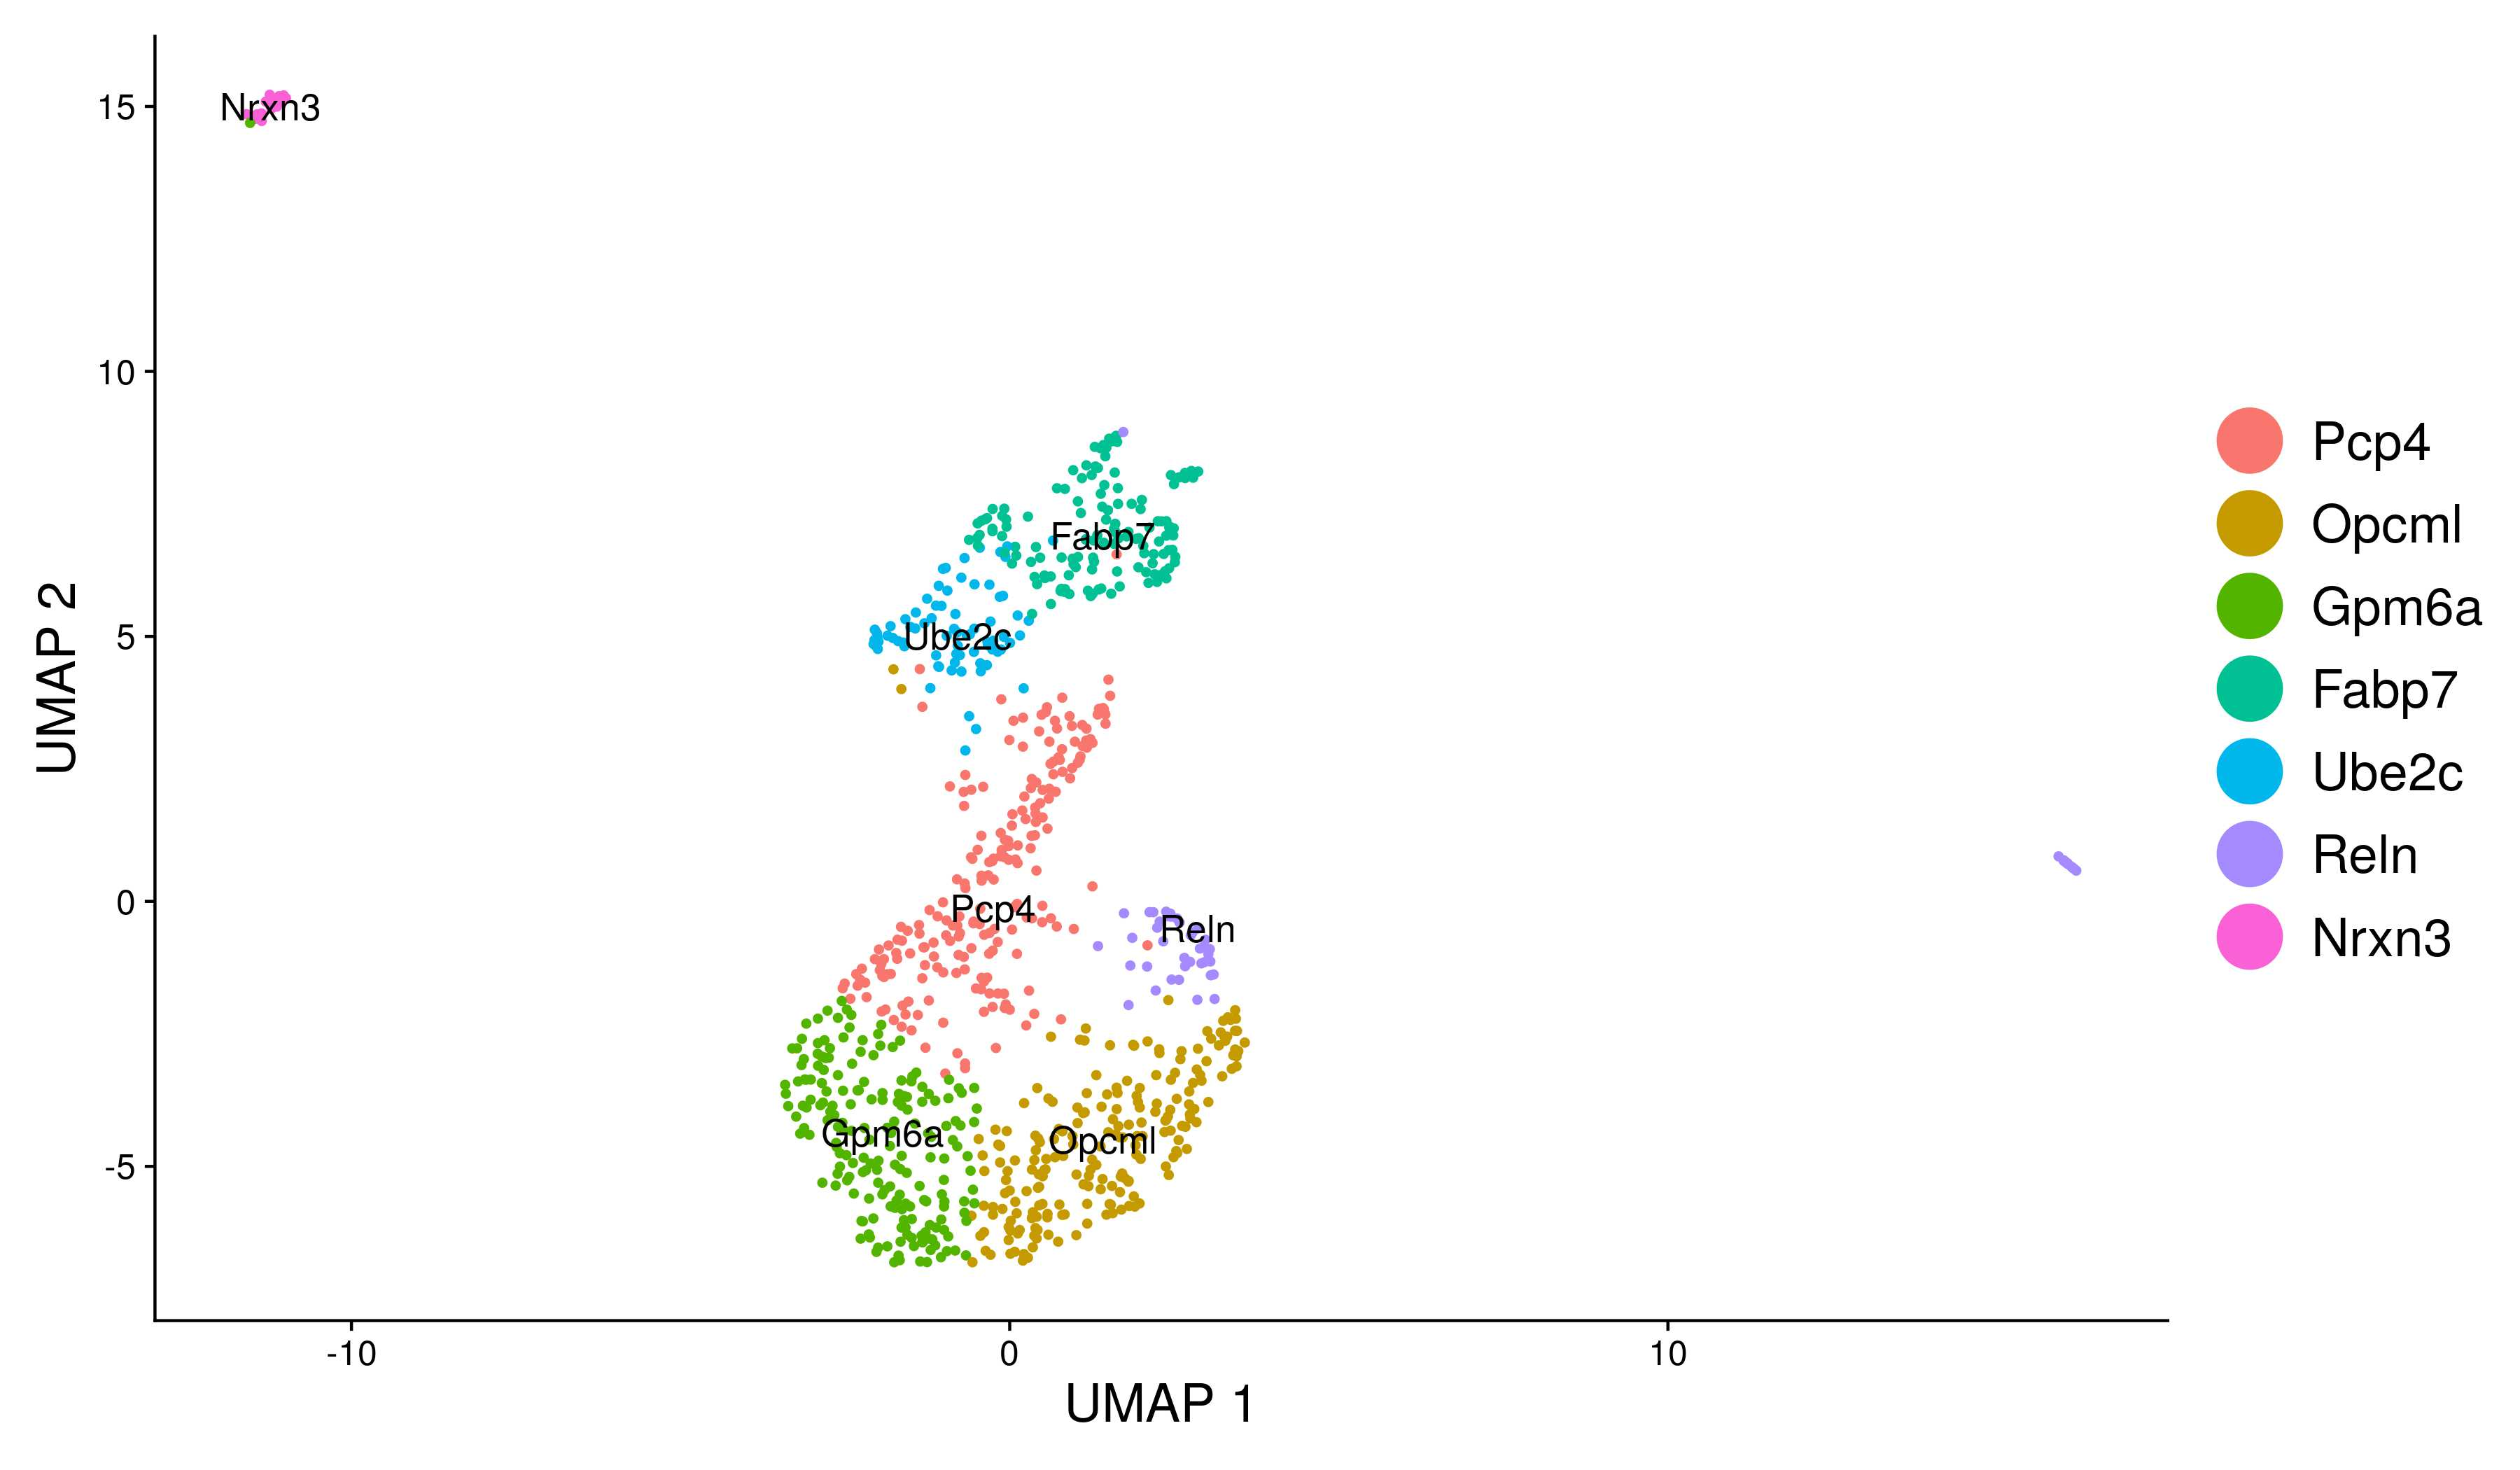
\includegraphics{output/neurons_900_umap.jpg}
\caption{named clusters}
\end{figure}

We observed that 1 marker gene in not enough to identify the cluster. To
do this we need more information about the dataset.

\begin{figure}
\centering
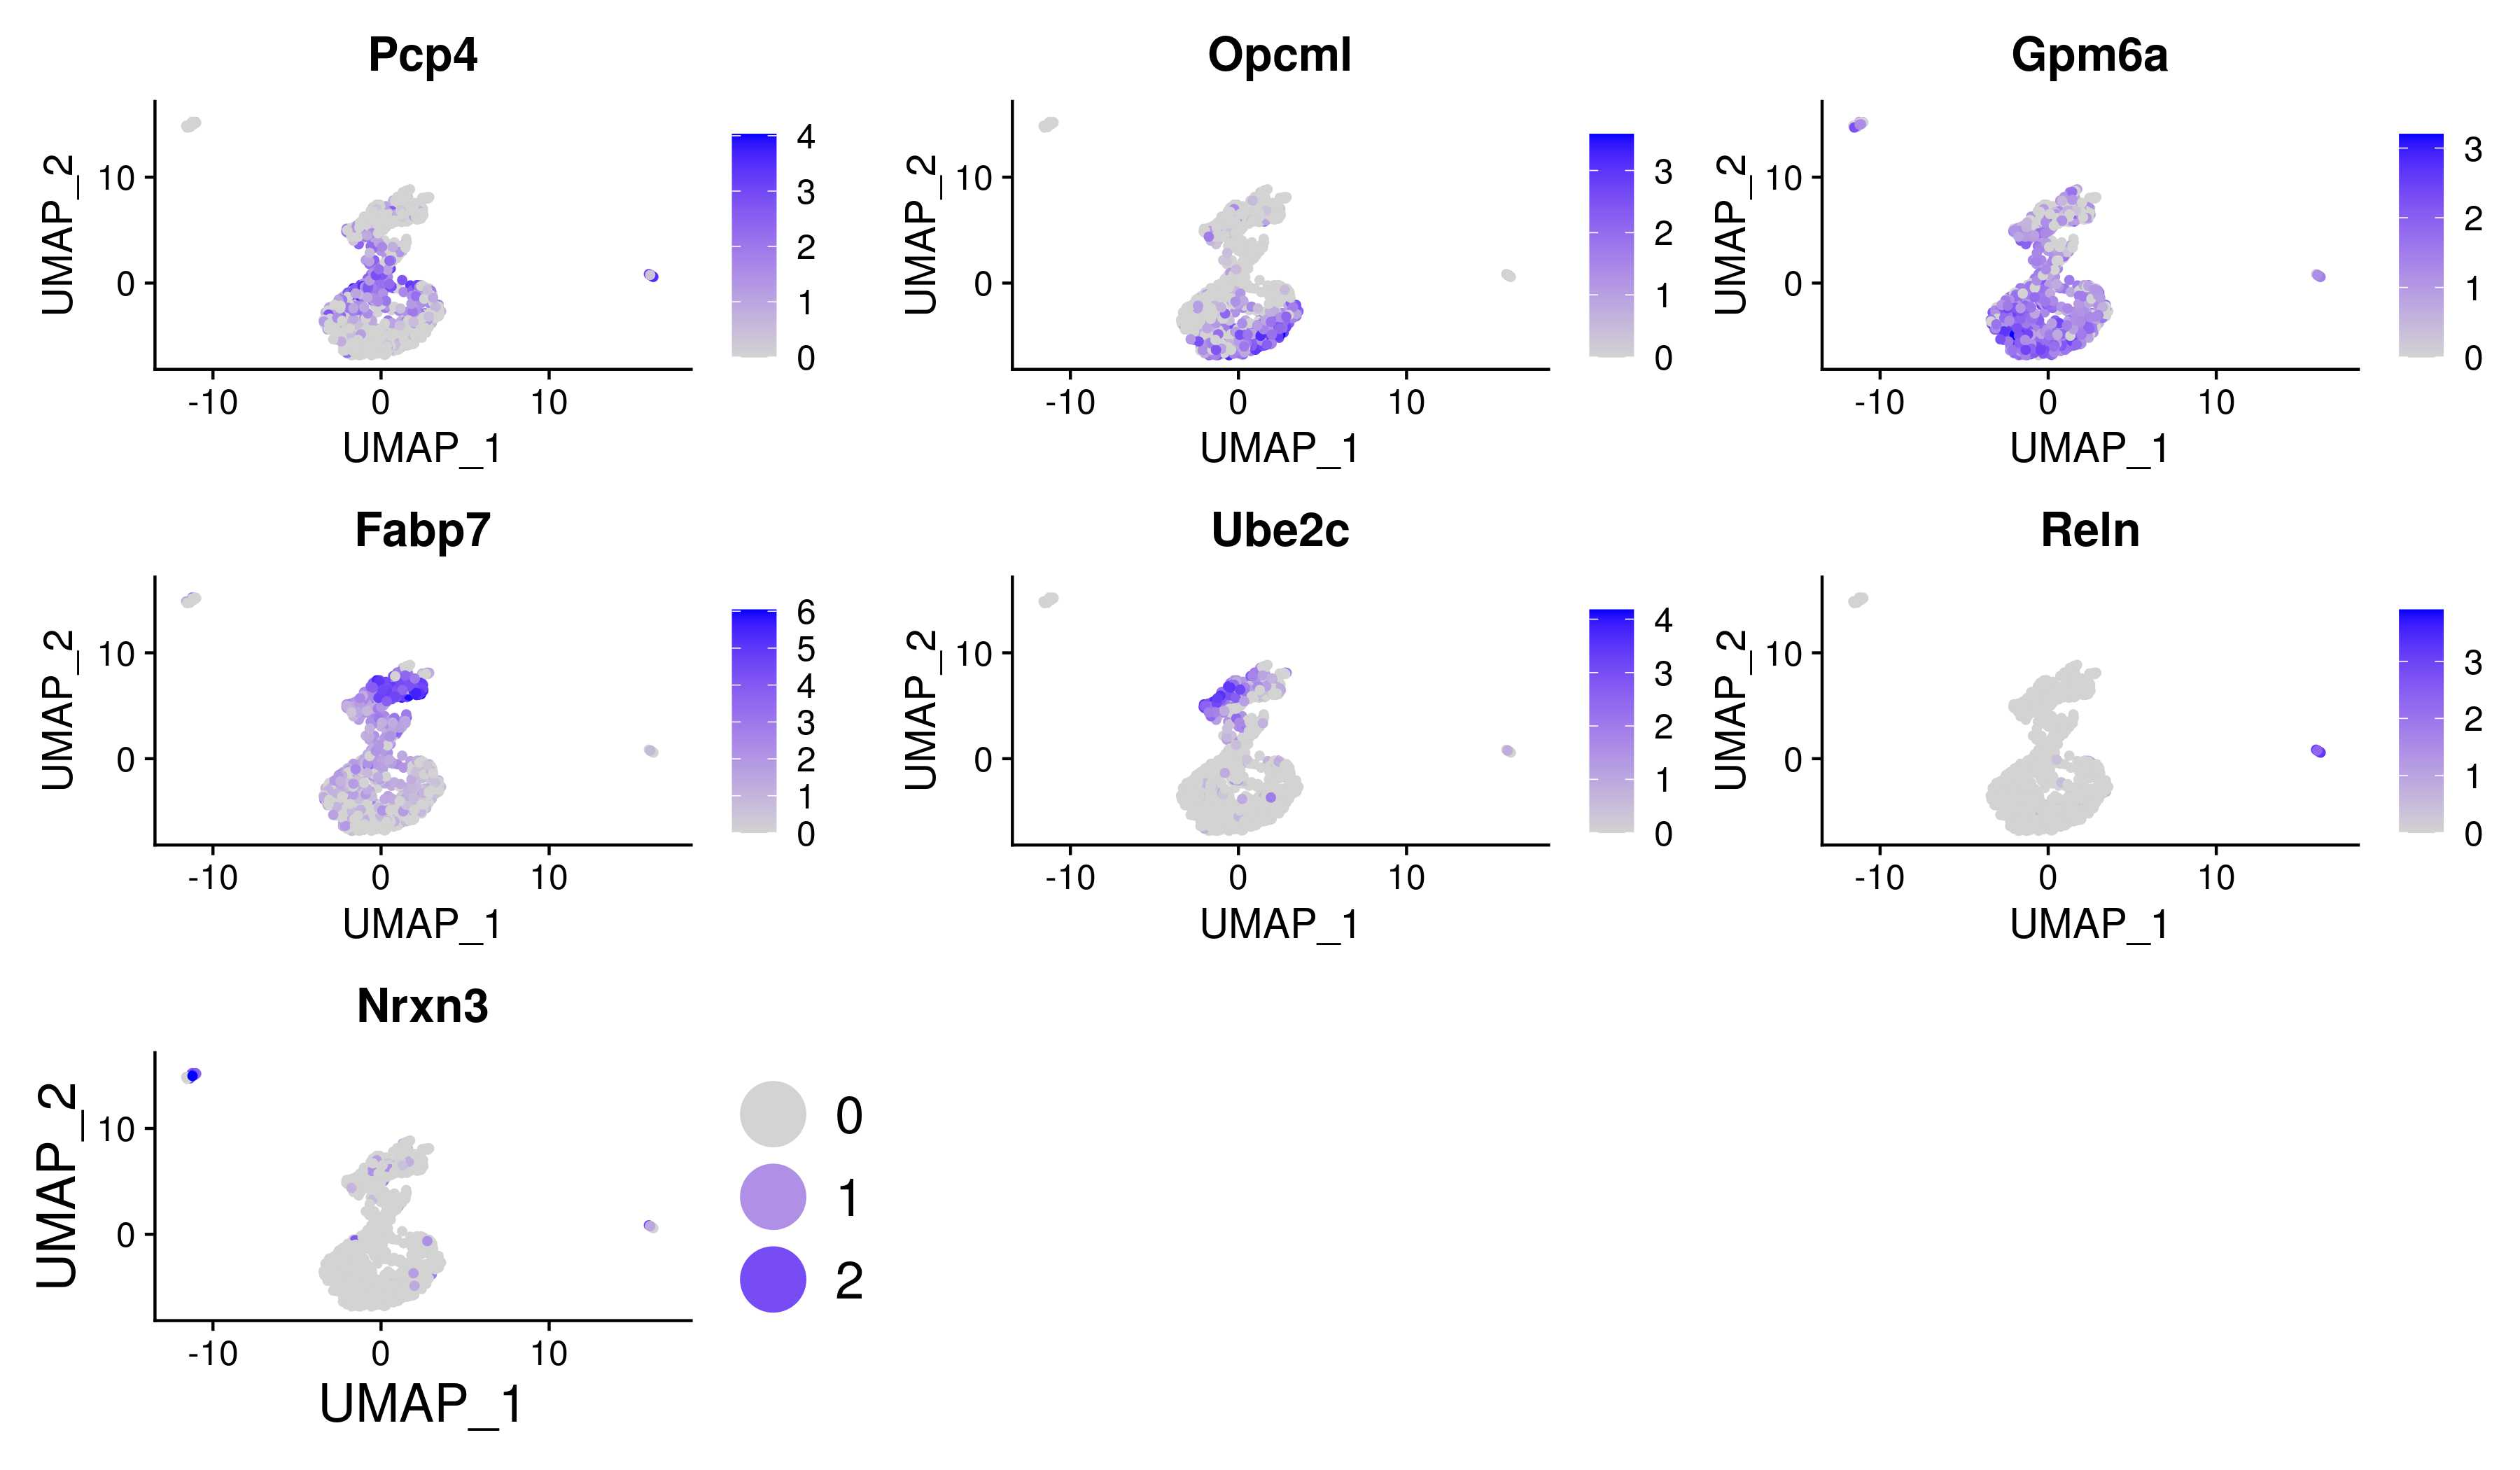
\includegraphics{output/neurons_900_FeaturePlot.jpg}
\caption{named clusters}
\end{figure}

We see that the genes are present in the corresponding clusters, but
there are limitations. For example the Rein gene is only present in part
of the cluster associated with it. It could also be necessary to fine
tune the settings to get a different number of clusters better suited to
the sample.

\hypertarget{discussion}{%
\subsection{Discussion}\label{discussion}}

We want to note, that we we focused on the workflow and not on the data
interpretation. To get more information we should combine our results
with biological information about the sample.

It is possible to reproduce the tutorial and use the method on a
different dataset. While it worked well there are some options to make
it easier. First the form of a notebook makes it difficult to see where
parameters are set and manual interventions are necessary. It is hard to
make changes without checking the whole code. In our opinion it would be
easier to write the code in functions or methods and use all variables
as function parameters. Notebooks are suited for presentation but are
limited for simply reusable code.

It would be possible to do the analysis in 2 well defined steps. Step 1
starting from pre-processing and ending with the analysis of the PCs. At
this point manual intervention is done. The rest of the analyses can be
performed without manual intervention in a second function or method.

\hypertarget{literature}{%
\subsubsection{Literature}\label{literature}}

Luecken and Theis 2019. Current best practices in single-cell RNA-seq
analysis: a tutorial. Molecular Systems Biology. 15(6):e8746.
doi:10.15252/msb.20188746.

Butler et al.~2018. Integrating single-cell transcriptomic data across
different conditions, technologies, and species. Nat Biotechnol.
36(5):411--420. doi:10.1038/nbt.4096.

Sandve et al.~2013. Ten Simple Rules for Reproducible Computational
Research. PLOS Computational Biology. 9(10):e1003285.
doi:10.1371/journal.pcbi.1003285.
